% Options for packages loaded elsewhere
\PassOptionsToPackage{unicode}{hyperref}
\PassOptionsToPackage{hyphens}{url}
\PassOptionsToPackage{dvipsnames,svgnames,x11names}{xcolor}
%
\documentclass[
  letterpaper,
  DIV=11,
  numbers=noendperiod]{scrartcl}
\usepackage{amsmath,amssymb}
\usepackage{lmodern}
\usepackage{iftex}
\ifPDFTeX
  \usepackage[T1]{fontenc}
  \usepackage[utf8]{inputenc}
  \usepackage{textcomp} % provide euro and other symbols
\else % if luatex or xetex
  \usepackage{unicode-math}
  \defaultfontfeatures{Scale=MatchLowercase}
  \defaultfontfeatures[\rmfamily]{Ligatures=TeX,Scale=1}
\fi
% Use upquote if available, for straight quotes in verbatim environments
\IfFileExists{upquote.sty}{\usepackage{upquote}}{}
\IfFileExists{microtype.sty}{% use microtype if available
  \usepackage[]{microtype}
  \UseMicrotypeSet[protrusion]{basicmath} % disable protrusion for tt fonts
}{}
\makeatletter
\@ifundefined{KOMAClassName}{% if non-KOMA class
  \IfFileExists{parskip.sty}{%
    \usepackage{parskip}
  }{% else
    \setlength{\parindent}{0pt}
    \setlength{\parskip}{6pt plus 2pt minus 1pt}}
}{% if KOMA class
  \KOMAoptions{parskip=half}}
\makeatother
\usepackage{xcolor}
\IfFileExists{xurl.sty}{\usepackage{xurl}}{} % add URL line breaks if available
\IfFileExists{bookmark.sty}{\usepackage{bookmark}}{\usepackage{hyperref}}
\hypersetup{
  pdftitle={Informe final},
  colorlinks=true,
  linkcolor={blue},
  filecolor={Maroon},
  citecolor={Blue},
  urlcolor={Blue},
  pdfcreator={LaTeX via pandoc}}
\urlstyle{same} % disable monospaced font for URLs
\usepackage{color}
\usepackage{fancyvrb}
\newcommand{\VerbBar}{|}
\newcommand{\VERB}{\Verb[commandchars=\\\{\}]}
\DefineVerbatimEnvironment{Highlighting}{Verbatim}{commandchars=\\\{\}}
% Add ',fontsize=\small' for more characters per line
\usepackage{framed}
\definecolor{shadecolor}{RGB}{40,42,54}
\newenvironment{Shaded}{\begin{snugshade}}{\end{snugshade}}
\newcommand{\AlertTok}[1]{\textcolor[rgb]{1.00,0.33,0.33}{\textbf{#1}}}
\newcommand{\AnnotationTok}[1]{\textcolor[rgb]{1.00,0.47,0.78}{#1}}
\newcommand{\AttributeTok}[1]{\textcolor[rgb]{1.00,0.47,0.78}{#1}}
\newcommand{\BaseNTok}[1]{\textcolor[rgb]{0.74,0.58,0.98}{#1}}
\newcommand{\BuiltInTok}[1]{\textcolor[rgb]{0.55,0.91,0.99}{#1}}
\newcommand{\CharTok}[1]{\textcolor[rgb]{0.95,0.98,0.55}{#1}}
\newcommand{\CommentTok}[1]{\textcolor[rgb]{0.38,0.45,0.64}{#1}}
\newcommand{\CommentVarTok}[1]{\textcolor[rgb]{0.55,0.91,0.99}{#1}}
\newcommand{\ConstantTok}[1]{\textcolor[rgb]{0.74,0.58,0.98}{\textbf{#1}}}
\newcommand{\ControlFlowTok}[1]{\textcolor[rgb]{1.00,0.47,0.78}{#1}}
\newcommand{\DataTypeTok}[1]{\textcolor[rgb]{0.55,0.91,0.99}{\textit{#1}}}
\newcommand{\DecValTok}[1]{\textcolor[rgb]{0.74,0.58,0.98}{#1}}
\newcommand{\DocumentationTok}[1]{\textcolor[rgb]{1.00,0.72,0.42}{#1}}
\newcommand{\ErrorTok}[1]{\textcolor[rgb]{1.00,0.33,0.33}{\underline{#1}}}
\newcommand{\ExtensionTok}[1]{\textcolor[rgb]{0.55,0.91,0.99}{#1}}
\newcommand{\FloatTok}[1]{\textcolor[rgb]{0.74,0.58,0.98}{#1}}
\newcommand{\FunctionTok}[1]{\textcolor[rgb]{0.31,0.98,0.48}{#1}}
\newcommand{\ImportTok}[1]{\textcolor[rgb]{1.00,0.47,0.78}{#1}}
\newcommand{\InformationTok}[1]{\textcolor[rgb]{0.95,0.98,0.55}{#1}}
\newcommand{\KeywordTok}[1]{\textcolor[rgb]{1.00,0.47,0.78}{#1}}
\newcommand{\NormalTok}[1]{\textcolor[rgb]{0.97,0.97,0.95}{#1}}
\newcommand{\OperatorTok}[1]{\textcolor[rgb]{0.97,0.97,0.95}{#1}}
\newcommand{\OtherTok}[1]{\textcolor[rgb]{0.31,0.98,0.48}{#1}}
\newcommand{\PreprocessorTok}[1]{\textcolor[rgb]{1.00,0.47,0.78}{#1}}
\newcommand{\RegionMarkerTok}[1]{\textcolor[rgb]{0.55,0.91,0.99}{#1}}
\newcommand{\SpecialCharTok}[1]{\textcolor[rgb]{1.00,0.47,0.78}{#1}}
\newcommand{\SpecialStringTok}[1]{\textcolor[rgb]{0.95,0.98,0.55}{#1}}
\newcommand{\StringTok}[1]{\textcolor[rgb]{0.95,0.98,0.55}{#1}}
\newcommand{\VariableTok}[1]{\textcolor[rgb]{0.55,0.91,0.99}{#1}}
\newcommand{\VerbatimStringTok}[1]{\textcolor[rgb]{0.95,0.98,0.55}{#1}}
\newcommand{\WarningTok}[1]{\textcolor[rgb]{1.00,0.33,0.33}{#1}}
\usepackage{longtable,booktabs,array}
\usepackage{calc} % for calculating minipage widths
% Correct order of tables after \paragraph or \subparagraph
\usepackage{etoolbox}
\makeatletter
\patchcmd\longtable{\par}{\if@noskipsec\mbox{}\fi\par}{}{}
\makeatother
% Allow footnotes in longtable head/foot
\IfFileExists{footnotehyper.sty}{\usepackage{footnotehyper}}{\usepackage{footnote}}
\makesavenoteenv{longtable}
\usepackage{graphicx}
\makeatletter
\def\maxwidth{\ifdim\Gin@nat@width>\linewidth\linewidth\else\Gin@nat@width\fi}
\def\maxheight{\ifdim\Gin@nat@height>\textheight\textheight\else\Gin@nat@height\fi}
\makeatother
% Scale images if necessary, so that they will not overflow the page
% margins by default, and it is still possible to overwrite the defaults
% using explicit options in \includegraphics[width, height, ...]{}
\setkeys{Gin}{width=\maxwidth,height=\maxheight,keepaspectratio}
% Set default figure placement to htbp
\makeatletter
\def\fps@figure{htbp}
\makeatother
\setlength{\emergencystretch}{3em} % prevent overfull lines
\providecommand{\tightlist}{%
  \setlength{\itemsep}{0pt}\setlength{\parskip}{0pt}}
\setcounter{secnumdepth}{-\maxdimen} % remove section numbering
% Make \paragraph and \subparagraph free-standing
\ifx\paragraph\undefined\else
  \let\oldparagraph\paragraph
  \renewcommand{\paragraph}[1]{\oldparagraph{#1}\mbox{}}
\fi
\ifx\subparagraph\undefined\else
  \let\oldsubparagraph\subparagraph
  \renewcommand{\subparagraph}[1]{\oldsubparagraph{#1}\mbox{}}
\fi
\KOMAoption{captions}{tableheading}
\makeatletter
\makeatother
\makeatletter
\@ifpackageloaded{caption}{}{\usepackage{caption}}
\AtBeginDocument{%
\renewcommand*\contentsname{Table of contents}
\renewcommand*\listfigurename{List of Figures}
\renewcommand*\listtablename{List of Tables}
\renewcommand*\figurename{Figure}
\renewcommand*\tablename{Table}
}
\@ifpackageloaded{float}{}{\usepackage{float}}
\floatstyle{ruled}
\@ifundefined{c@chapter}{\newfloat{codelisting}{h}{lop}}{\newfloat{codelisting}{h}{lop}[chapter]}
\floatname{codelisting}{Listing}
\newcommand*\listoflistings{\listof{codelisting}{List of Listings}}
\makeatother
\makeatletter
\@ifpackageloaded{caption}{}{\usepackage{caption}}
\@ifpackageloaded{subcaption}{}{\usepackage{subcaption}}
\makeatother
\makeatletter
\makeatother
\ifLuaTeX
  \usepackage{selnolig}  % disable illegal ligatures
\fi

\title{Informe final}
\author{}
\date{2022-07-02}

\begin{document}
\maketitle

\renewcommand*\contentsname{Table of contents}
{
\hypersetup{linkcolor=}
\setcounter{tocdepth}{4}
\tableofcontents
}
\hypertarget{caruxe1tula}{%
\subsection{CARÁTULA}\label{caruxe1tula}}

\begin{itemize}
\item
  \textbf{Curso:} Análisis de Datos
\item
  \textbf{Profesor:} Stefany Neciosup
\item
  \textbf{Código del curso:} 1INF03
\item
  \textbf{Fecha de Entrega:} 02/07/2022
\item
  \textbf{Integrantes:}

  \begin{itemize}
  \tightlist
  \item
    Richle Gianotti, Renzo Ernesto - 20180368
  \item
    Cornejo Ramírez, Lucio Enrique - 20192058
  \item
    Vivas Alejandro, Claudia Mirela - 20141150
  \item
    Mejia Padilla, Andrea Adela - 20180824
  \end{itemize}
\end{itemize}

\hypertarget{introducciuxf3n}{%
\subsection{INTRODUCCIÓN}\label{introducciuxf3n}}

Para comprender la dinámica de la industria musical, antes que nada, es
necesario saber que no se trata de una sola, sino de varias,
estrechamente relacionadas entre sí, pero que surgen a partir de lógicas
y estructuras distintas. La industria musical en su conjunto vive de la
creación y la explotación de la propiedad intelectual musical.
Compositores y letristas crean canciones, letras y arreglos que se
interpretan en directo sobre el escenario, se graban y distribuyen a los
consumidores. Esta estructura básica ha dado lugar a tres industrias
musicales centrales: la discográfica, centrada en la grabación de música
y su distribución a los consumidores; la de las licencias musicales, que
sobre todo concede licencias a empresas para la difusión de
composiciones y arreglos; y, la música en vivo, centrada en producir y
promocionar espectáculos en directo, como conciertos, giras, etc.

El desarrollo de la Ciencia de Datos permite el uso de data para mejorar
la toma de decisiones en el sector público y privado. La industria
musical no es la excepción, pues también existe un interés por generar
nuevas canciones populares, con el fin de recuperar los costos de
produccion de una canción y maximizar márgenes de ganancia. En base a
tal problemática, se desarrolla el presente trabajo con el objetivo de
desarrollar un modelo que logre predecir la propularidad de las
canciones futuras, como resultado de un análisis de las variables que
influyan de manera positiva o negativa en la popularidad de las
canciones. De esta forma, el modelo análitico podrá ser utilizado para
predecir la popularidad de las canciones, lo cual ayudará a tomar
decisiones de manera más efectiva.

Estas son algunas de las interrogantes que se explorarán en este
trabajo:

\begin{itemize}
\tightlist
\item
  ¿Qué características en común tienen las canciones más populares de
  Spotify?
\item
  ¿Existe una correlación entre la popularidad y alguna característica
  de las canciones?
\item
  ¿Cuánto debe durar un track según los estándares de la actualidad?
\end{itemize}

\hypertarget{capuxedtulo-i-comprensiuxf3n-del-negocio-estudio}{%
\subsection{CAPÍTULO I: COMPRENSIÓN DEL NEGOCIO /
ESTUDIO}\label{capuxedtulo-i-comprensiuxf3n-del-negocio-estudio}}

\hypertarget{descripciuxf3n-del-problema}{%
\subsubsection{Descripción del
problema}\label{descripciuxf3n-del-problema}}

Se puede tener una percepción de las canciones más populares a nivel
mundial observando la cantidad de reproducciones de cada canción en las
plataformas musicales, lo cual se traduce en mayores ganancias para los
artistas, empresas discográficas y todas las personas detrás del
lanzamiento de una canción. En este contexto, la popularidad es la
variable que determina los márgenes de ganancias de la industria
musical, así un problema y preocupación recurrente, dentro de la
industria musical, es generar canciones populares

\hypertarget{objetivo-del-negocioestudio}{%
\subsubsection{Objetivo del
negocio/estudio}\label{objetivo-del-negocioestudio}}

Nuestro objetivo principal es desarrollar un modelo que logre predecir
si una canción será popular o no antes de ser lanzada al mercado.
Además, nuestro objetivo secundario, es conocer las características que
hacen popular a una canción.

\hypertarget{variable-objetivo-para-el-negocio}{%
\subsubsection{Variable objetivo para el
negocio}\label{variable-objetivo-para-el-negocio}}

\begin{itemize}
\tightlist
\item
  ``Popularity'' es la variable objetivo.
\end{itemize}

\hypertarget{capuxedtulo-ii-fuentes-de-informaciuxf3n}{%
\subsection{CAPÍTULO II: FUENTES DE
INFORMACIÓN}\label{capuxedtulo-ii-fuentes-de-informaciuxf3n}}

\hypertarget{origen-de-los-datos-del-proyecto}{%
\subsubsection{Origen de los datos del
proyecto}\label{origen-de-los-datos-del-proyecto}}

El dataset que empleamos lo descargamos de
\href{https://www.kaggle.com/datasets/yamaerenay/spotify-dataset-19212020-600k-tracks?resource=download}{Kaggle}
de donde usamos el archivo\textbf{tracks.csv}. Como se describe en el
sitio web del link previo, el dataset \textbf{tracks.csv} se obtuvo vía
el \href{https://developer.spotify.com/documentation/web-api/}{API
oficial de \textbf{Spotify}}. Esta permite descargar, características de
las canciones disponibles en la plataforma tales como su duración en
milisegundos, volumen, qué tan bailable es, etc.

Así, cada fila en \textbf{tracks.csv} representa a una canción diferente
en Spotify, y, las columnas del dataset representan características
─variables─ asociadas a cada canción.

\hypertarget{descripciuxf3n-del-universo-y-muestra}{%
\subsubsection{Descripción del universo y
muestra}\label{descripciuxf3n-del-universo-y-muestra}}

El \textbf{universo} de datos está conformado por el conjunto de
canciones de Spotify disponibles en el instante de tiempo en que se
descargó el dataset, vía la API oficial de Spotify. En la
\href{https://www.kaggle.com/datasets/yamaerenay/spotify-dataset-19212020-600k-tracks?resource=download}{página
web}, fuente de descargamos la data, se menciona que las canciones
extraídas fueron publicadas entre los años 1921 y 2020. Asimismo, la
muestra tiene y 20 columnas.

En ese sentido, la \textbf{muestra} consiste en el conjunto de canciones
de Spotify de las cuales tenemos información en las filas del dataset
descargado ─586672 observaciones ─ y 20 columnas. No obstante, esta
muestra es arbitraria, ya que no se especifica la estrategia de
muestreo. A nivel de grupo, discutimos la importancia del muestro y
concluimos que, para realizar un análisis riguroso necesitaremos
realizar una muestro multietápico diseñado por nosotros mismo, pero por
la limitación de tiempo, seguiremos usando la data original.

La arbitrariedad de la muestra se refleja en algunas fallas que
detectamos en la etapa de exploración de los datos, pues tras analizar
la data descargada, observamos que los años de lanzamiento de las
canciones se encuentran en el rango de 1900 a 2021. Es decir, existen,
observaciones que están fuera del rango de años especificados en la
fuente secundaria ─Kaggle─. Específicamente encontramos que, el año de
lanzamiento de una canción del dataset fue en 1990, sin embargo, tras
realizar una pequeña una búsqueda web, hallamos que la banda que creó
tal canción aún sigue activa. En otras palabras, es imposible que, en
caso la banda lanzará la canción en 1990, siga activa.

Es plausible afirmar que la data que disponemos tenga algunas fallas, lo
cual debería subsanarse para obtener un mejor resultado. Durante las
reuniones de equipo, evaluamos scrappear las canciones de Spotify
empleando el API oficial de Spotify para obtener la data de las
canciones cuyo identificador ya se posee, gracias al dataset descargado.
Esto último con el fin de crear un nuevo dataset, ahora sin errores, con
el cual trabajaríamos como base datos de este proyecto. También
evaluamos descartar a las filas donde encontremos errores como el
mencionado previamente respecto a la fecha de publicación de la canción.
No obstante, por limitaciones de tiempo, llevamos al consenso de
continuar el dataset original.

Por otro lado, la muestra contiene las siguientes columnas:

\begin{Shaded}
\begin{Highlighting}[]
\CommentTok{\# Data numérica previo a imputación}
\NormalTok{dfnum\_pre\_imp }\OperatorTok{=}\NormalTok{ pd.read\_csv(}\StringTok{"../datos/dfnum\_pre\_imp.csv"}\NormalTok{)}

\CommentTok{\# Data categórica previo a transformación de variables}
\NormalTok{dfcat\_pre\_trans }\OperatorTok{=}\NormalTok{ pd.read\_csv(}\StringTok{"../datos/dfcat.csv"}\NormalTok{)}
\end{Highlighting}
\end{Shaded}

\begin{Shaded}
\begin{Highlighting}[]
\CommentTok{\# Tabla de descripción básica de las variables numéricas}
\NormalTok{DT}\SpecialCharTok{::}\FunctionTok{datatable}\NormalTok{(py}\SpecialCharTok{$}\NormalTok{temp\_df)}
\end{Highlighting}
\end{Shaded}

\begin{figure}[H]

{\centering 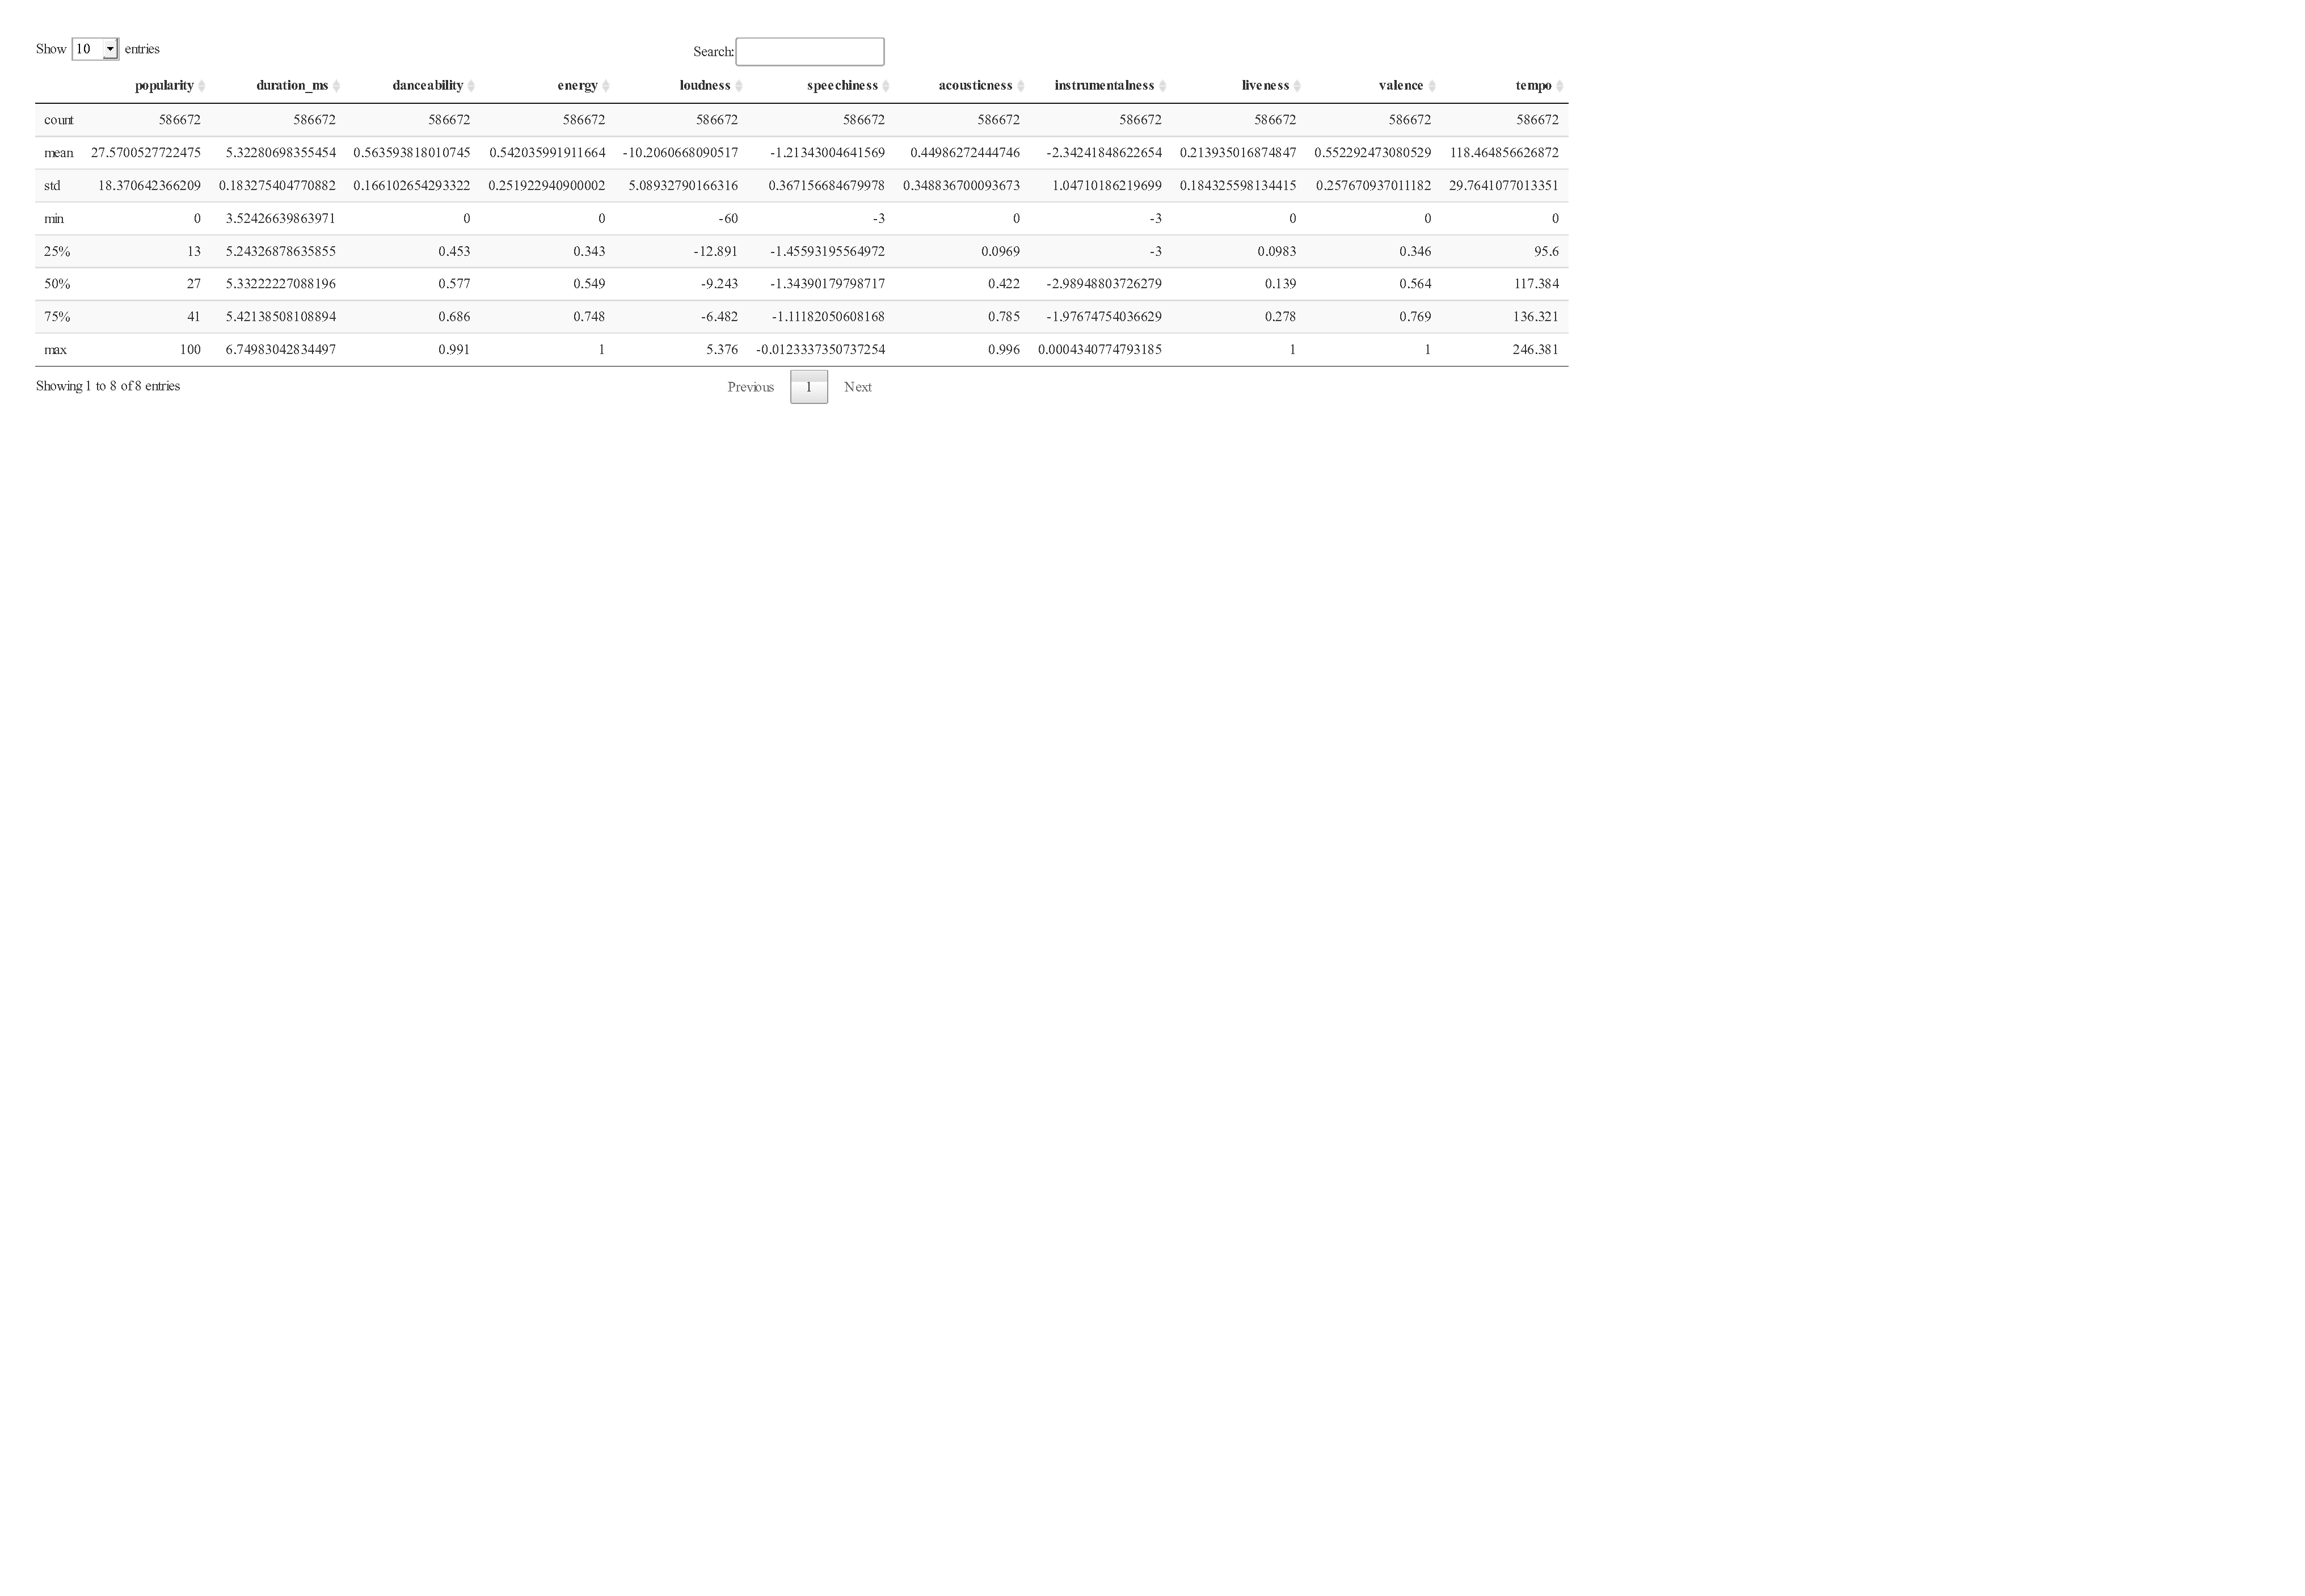
\includegraphics{informe_01_files/figure-pdf/unnamed-chunk-6-1.pdf}

}

\end{figure}

A continuación, graficamos la densidad de las variables numéricas,
además de rectas verticales para representar la media (rojo), mediana
(verde), cuartiles 1 y 3 (negro); y los whiskers definidos, en amarillo.

\hypertarget{loudness}{%
\paragraph{Loudness}\label{loudness}}

Describe la sonoridad general de una pista en decibeles. Los valores de
sonoridad se promedian en toda la pista y son útiles para comparar la
sonoridad relativa de las pistas. La sonoridad es la cualidad de un
sonido que es el principal correlato psicológico de la fuerza física
(amplitud). Los valores suelen oscilar entre -60 y 0 db.

\begin{verbatim}
C:\Python39\lib\site-packages\seaborn\distributions.py:2619: FutureWarning: `distplot` is a deprecated function and will be removed in a future version. Please adapt your code to use either `displot` (a figure-level function with similar flexibility) or `histplot` (an axes-level function for histograms).
  warnings.warn(msg, FutureWarning)
\end{verbatim}

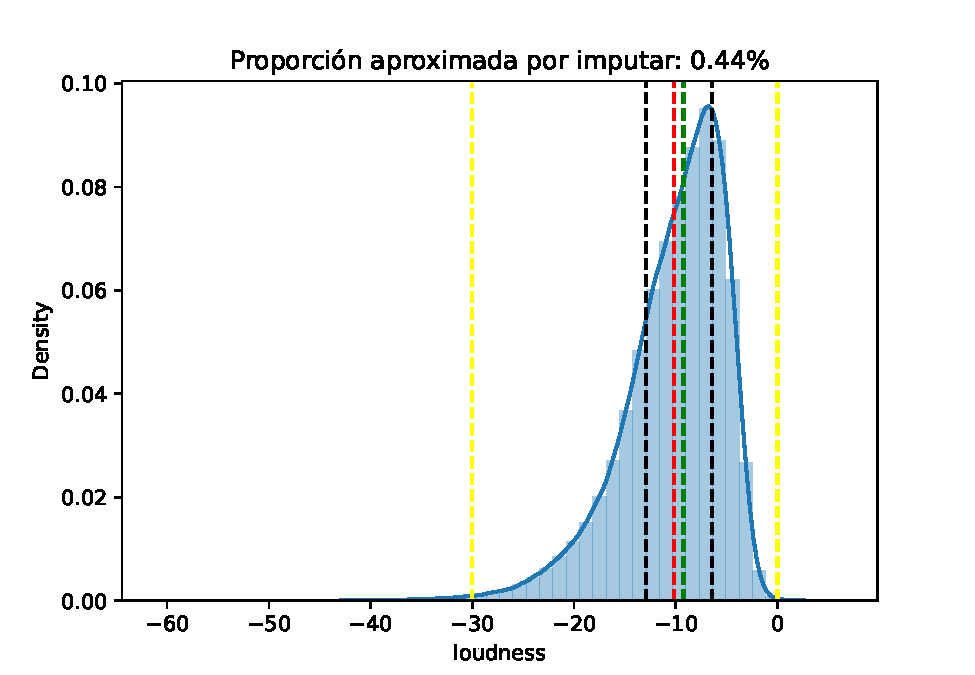
\includegraphics{informe_01_files/figure-pdf/unnamed-chunk-10-1.pdf}

\hypertarget{instrumentalness}{%
\paragraph{Instrumentalness}\label{instrumentalness}}

Predice si una pista no contiene voces. Los sonidos ``Ooh'' y ``aah'' se
consideran instrumentales en este contexto. Las pistas de rap o de
palabras habladas son claramente ``vocales''. Cuanto más se acerque el
valor de instrumentalización a 1,0, mayor será la probabilidad de que la
pista no tenga contenido vocal. Los valores superiores a 0,5 representan
pistas instrumentales, pero la confianza es mayor a medida que el valor
se acerca a 1,0.

\begin{verbatim}
C:\Python39\lib\site-packages\seaborn\distributions.py:2619: FutureWarning: `distplot` is a deprecated function and will be removed in a future version. Please adapt your code to use either `displot` (a figure-level function with similar flexibility) or `histplot` (an axes-level function for histograms).
  warnings.warn(msg, FutureWarning)
\end{verbatim}

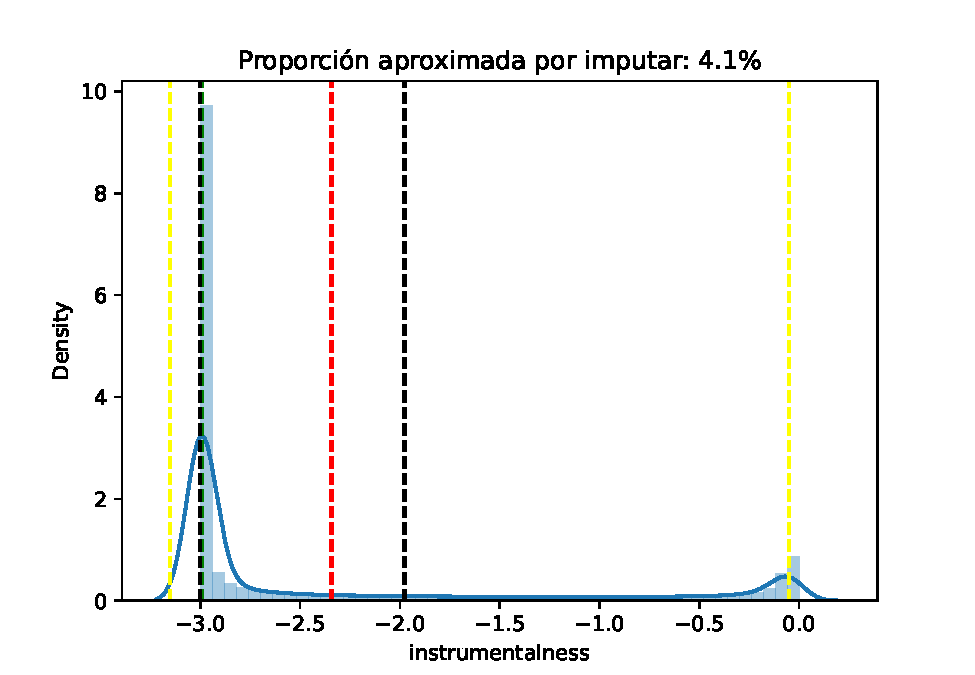
\includegraphics{informe_01_files/figure-pdf/unnamed-chunk-12-3.pdf}

\hypertarget{liveness}{%
\paragraph{Liveness}\label{liveness}}

Detecta la presencia de una audiencia en la grabación. Valores más altos
de liveness representan una probabilidad incrementada de que la pista
haya sido realizada en vivo. Un valor de 0.8 provee una probabilidad
fuerte de que la pista sea en vivo.

\begin{verbatim}
C:\Python39\lib\site-packages\seaborn\distributions.py:2619: FutureWarning: `distplot` is a deprecated function and will be removed in a future version. Please adapt your code to use either `displot` (a figure-level function with similar flexibility) or `histplot` (an axes-level function for histograms).
  warnings.warn(msg, FutureWarning)
\end{verbatim}

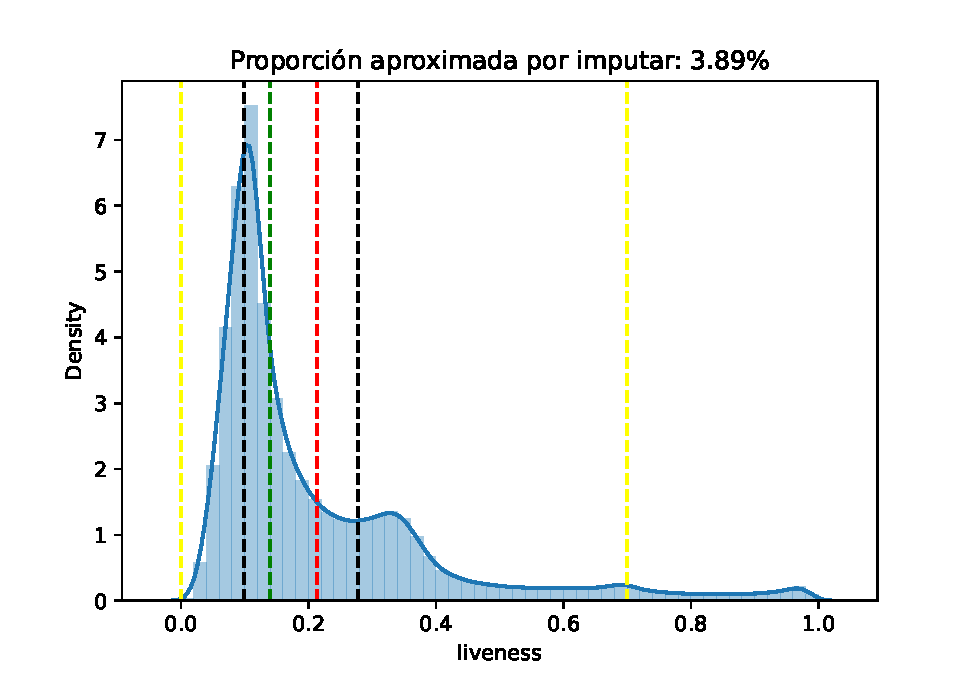
\includegraphics{informe_01_files/figure-pdf/unnamed-chunk-14-5.pdf}

\hypertarget{valence}{%
\paragraph{Valence}\label{valence}}

Es medida desde 0.0 hasta 1.0 que describe la positividad musical
expresada por la pista. Las pistas con un sonido de alta valence suenan
más positivos (e.g., felices, alegres, eufóricos), mientras que las
pistas con una baja valence suenan más negativas (e.g., tristes,
deprimentes, enojadas).

\begin{verbatim}
C:\Python39\lib\site-packages\seaborn\distributions.py:2619: FutureWarning: `distplot` is a deprecated function and will be removed in a future version. Please adapt your code to use either `displot` (a figure-level function with similar flexibility) or `histplot` (an axes-level function for histograms).
  warnings.warn(msg, FutureWarning)
\end{verbatim}

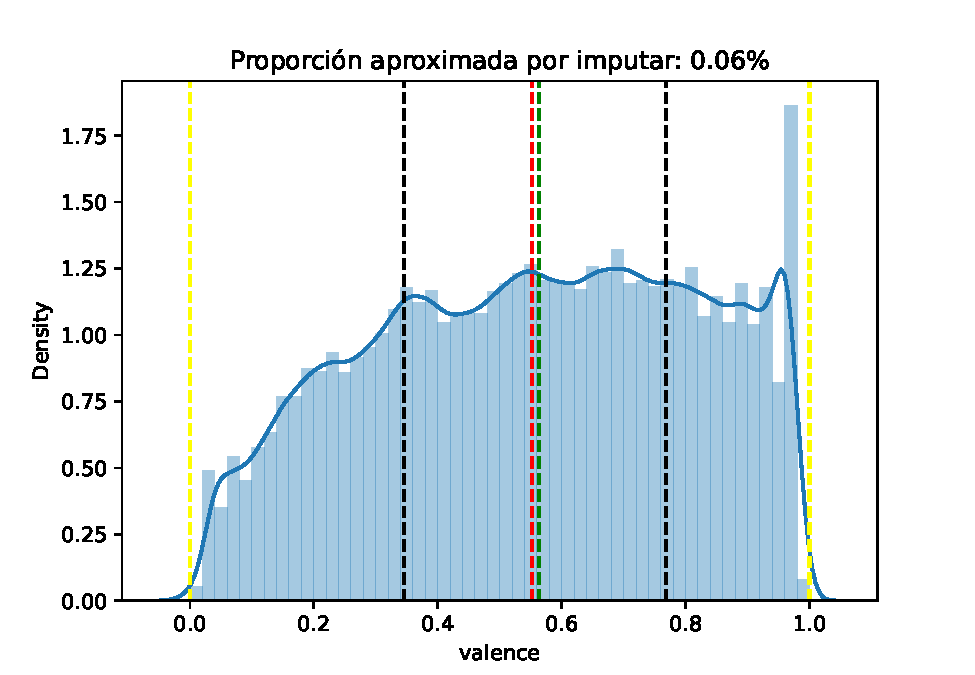
\includegraphics{informe_01_files/figure-pdf/unnamed-chunk-16-7.pdf}

\hypertarget{tempo}{%
\paragraph{Tempo}\label{tempo}}

Es el tempo general estimado de una pista en beats por minutos (BPM, por
sus siglas en inglés). En terminología musical, el tempo es la velocidad
o ritmo de una pieza dada y se deriva directamente de una duración
promedio de beat.

\begin{verbatim}
C:\Python39\lib\site-packages\seaborn\distributions.py:2619: FutureWarning: `distplot` is a deprecated function and will be removed in a future version. Please adapt your code to use either `displot` (a figure-level function with similar flexibility) or `histplot` (an axes-level function for histograms).
  warnings.warn(msg, FutureWarning)
\end{verbatim}

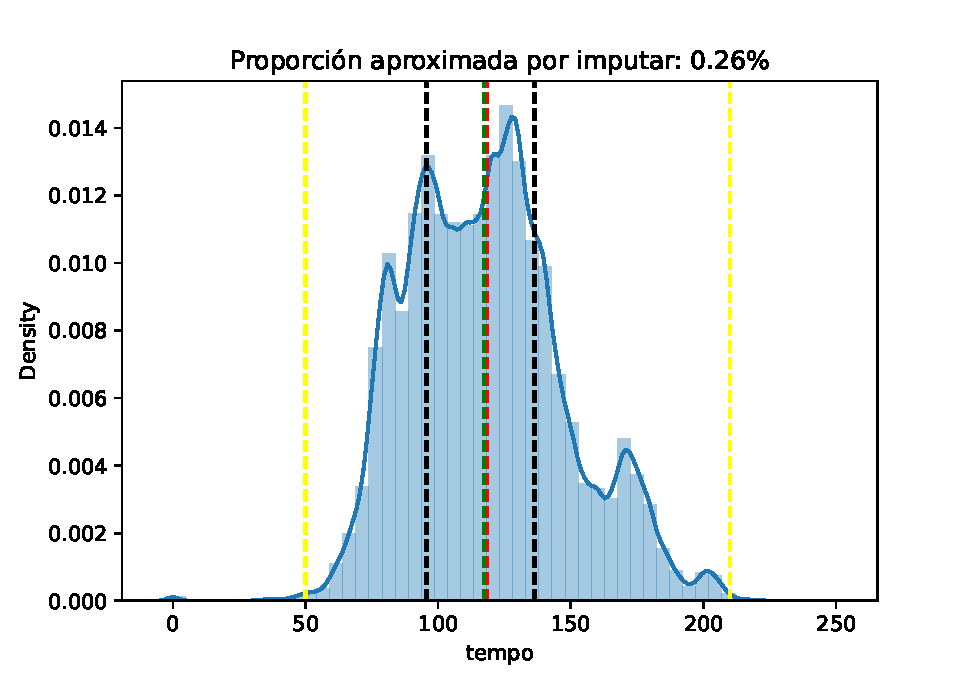
\includegraphics{informe_01_files/figure-pdf/unnamed-chunk-18-9.pdf}

\hypertarget{duration_ms}{%
\paragraph{Duration\_ms}\label{duration_ms}}

Es la duración de una pieza en milisegundos. Respecto a la distribución
de esta variable, se observa que la distribución de los datos es en
principio aparentemente degenerada (los datos están virtual o totalmente
reunidos en un punto). No obstante, tal aparente degeneración se explica
por el hecho de que existe una serie de piezas cuya duración puede ser
extremadamente larga.

\begin{verbatim}
C:\Python39\lib\site-packages\seaborn\distributions.py:2619: FutureWarning: `distplot` is a deprecated function and will be removed in a future version. Please adapt your code to use either `displot` (a figure-level function with similar flexibility) or `histplot` (an axes-level function for histograms).
  warnings.warn(msg, FutureWarning)
\end{verbatim}

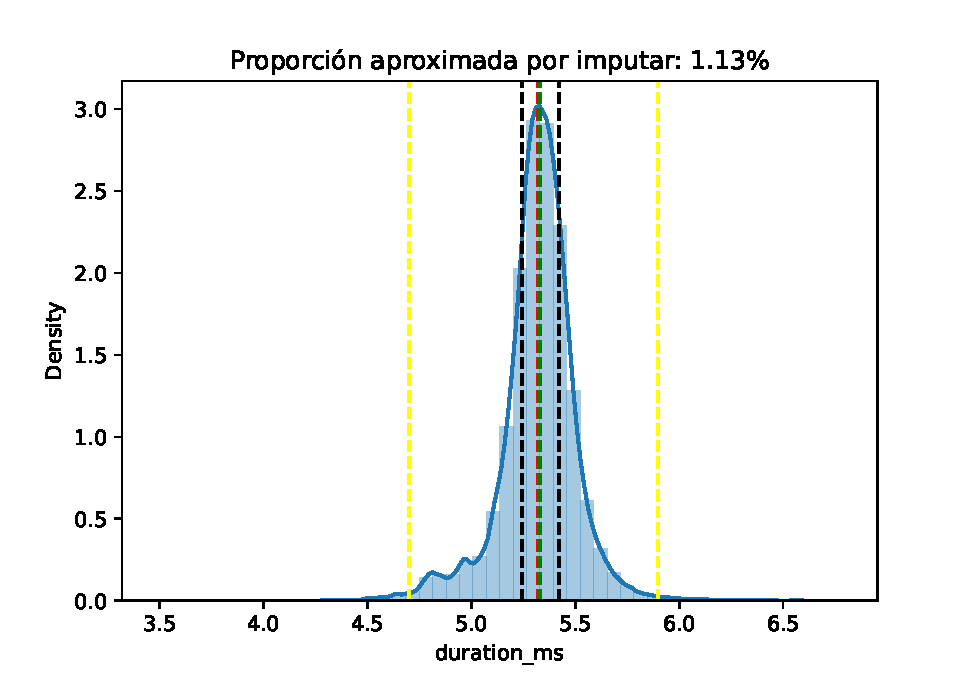
\includegraphics{informe_01_files/figure-pdf/unnamed-chunk-20-11.pdf}

\hypertarget{danceability}{%
\paragraph{Danceability}\label{danceability}}

La danceability describe qué tan adecuada es una pista para bailar,
basada en una combinación de elementos musicales incluyendo el tempo, la
estabilidad rítmica (rhythm stability), la fuerza del beat (beat
strength), y una regularidad general. Un valor de 0.0 es menos danceable
1.0 es máximamente danceable.

\begin{verbatim}
C:\Python39\lib\site-packages\seaborn\distributions.py:2619: FutureWarning: `distplot` is a deprecated function and will be removed in a future version. Please adapt your code to use either `displot` (a figure-level function with similar flexibility) or `histplot` (an axes-level function for histograms).
  warnings.warn(msg, FutureWarning)
\end{verbatim}

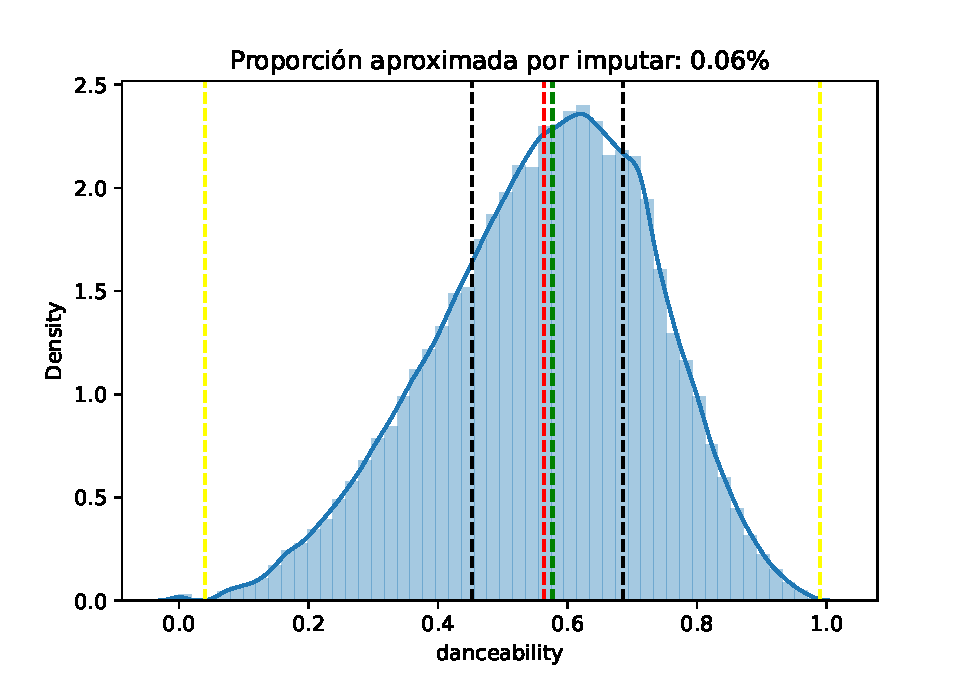
\includegraphics{informe_01_files/figure-pdf/unnamed-chunk-22-13.pdf}

\hypertarget{energy}{%
\paragraph{Energy}\label{energy}}

La energía es una medida desde 0.0 a 1.0 y representa una medida
perceptiva de intensidad y actividad. Típicamente, las pistas
energéticas se sienten rápidas, de volumen alto (loud), y ruidosas. Por
ejemplo, el death metal tiene una alta energía, mientras que el preludio
de Bach da un puntaje bajo en la escala. Características perceptivas
contribuyen a este atributo incluyen rango dinámico, el volumen
percibió, el timbre, el onset rate, y la entropía general.

\begin{verbatim}
C:\Python39\lib\site-packages\seaborn\distributions.py:2619: FutureWarning: `distplot` is a deprecated function and will be removed in a future version. Please adapt your code to use either `displot` (a figure-level function with similar flexibility) or `histplot` (an axes-level function for histograms).
  warnings.warn(msg, FutureWarning)
\end{verbatim}

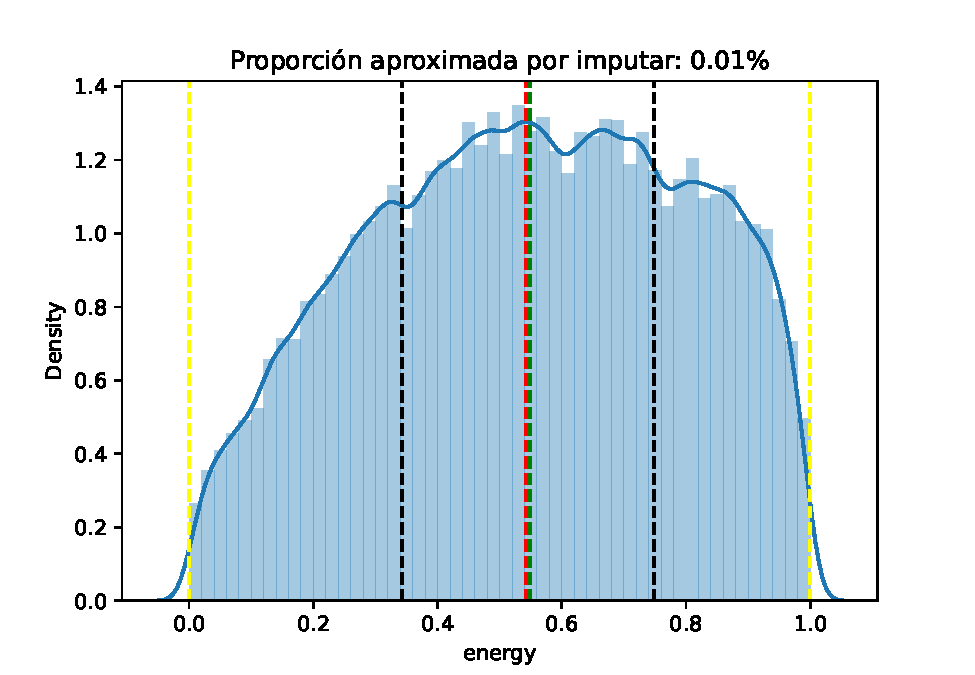
\includegraphics{informe_01_files/figure-pdf/unnamed-chunk-24-15.pdf}

\hypertarget{speechiness}{%
\paragraph{Speechiness}\label{speechiness}}

Esta variableetecta la presencia de palabras habladas en una pieza.
Mientras más contenido hablado presenta una grabación (e.g., talk show,
audio book, poesía), más cercano a 1.0 será el valor del atributo. Los
valores superiores a 0.66 describen piezas que probablemente estén
hechas enteramente de palabras habladas. Valores entre 0.33 y 0.66
describen piezas que podrías contener tanto música como una parte oral,
ya sea en secciones o en capas, incluyendo casos como el rap. Valores
menores a 0.33 con mayor probabilidad representan múscia y otras piezas
non-speech-like.

\begin{verbatim}
C:\Python39\lib\site-packages\seaborn\distributions.py:2619: FutureWarning: `distplot` is a deprecated function and will be removed in a future version. Please adapt your code to use either `displot` (a figure-level function with similar flexibility) or `histplot` (an axes-level function for histograms).
  warnings.warn(msg, FutureWarning)
\end{verbatim}

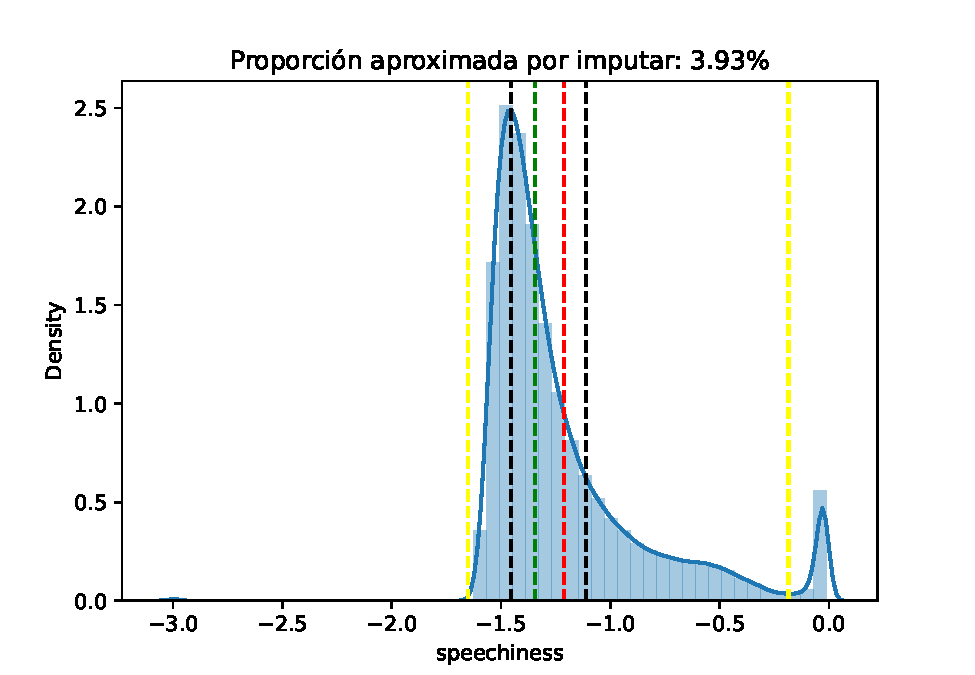
\includegraphics{informe_01_files/figure-pdf/unnamed-chunk-26-17.pdf}

\hypertarget{acousticness}{%
\paragraph{Acousticness}\label{acousticness}}

Una medida de confianza desde 0.0 hasta 1.0 sobre si la pieza es
acústica. 1.0 representa alta confianza en que la pieza es acústica
(\textgreater=0 \textbar{} \textless= 1).

\begin{verbatim}
C:\Python39\lib\site-packages\seaborn\distributions.py:2619: FutureWarning: `distplot` is a deprecated function and will be removed in a future version. Please adapt your code to use either `displot` (a figure-level function with similar flexibility) or `histplot` (an axes-level function for histograms).
  warnings.warn(msg, FutureWarning)
\end{verbatim}

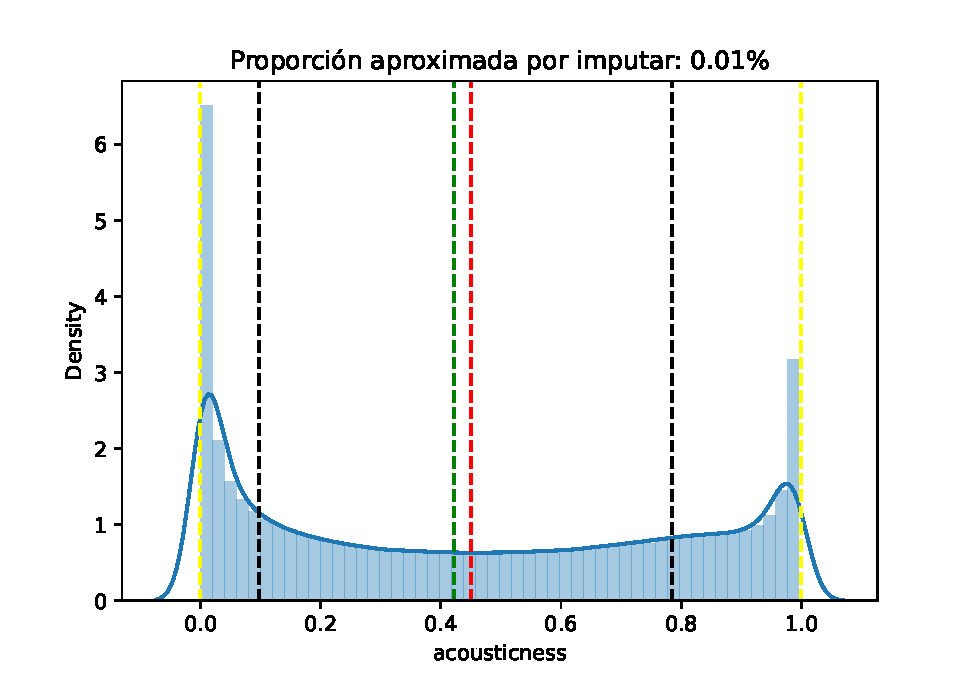
\includegraphics{informe_01_files/figure-pdf/unnamed-chunk-28-19.pdf}

\hypertarget{descripciuxf3n-y-entendimiento-de-variables}{%
\subsubsection{Descripción y entendimiento de
variables}\label{descripciuxf3n-y-entendimiento-de-variables}}

Esta sección del capítulo dos la hemos desarrollado en el
\textbf{Jupyter notebook} presentado para este informe, así que no
incluiremos aquella descripción en este archivo.

La exploraricón de las variables ha sido realizada mediante
\href{https://lucio-cornejo.shinyapps.io/chapter-II-dashboard-INF03/}{esta}
aplicación web. Así, encontramos los siguientes patrones en la data:

\begin{itemize}
\tightlist
\item
  A partir de 1950, para décadas cada vez más recientes, existe una
  mayor proporción de canciones que presentan valores cada vez más
  grandes de popularidad.
\item
  Para décadas más recientes, las canciones más populares tienden a ser
  aquellas cuya longitud del nombre está entre 3 y 10 caracteres.
\end{itemize}

\hypertarget{capuxedtulo-iii-preprocesamiento-de-datos}{%
\subsection{CAPÍTULO III: PREPROCESAMIENTO DE
DATOS}\label{capuxedtulo-iii-preprocesamiento-de-datos}}

En ese capitulo se detalla el proceso de preprocesamiento de los datos.
Donde, la variable popularity es la variable dependiente del estudio por
lo cual esta variable no debe pasar por ningún tratamiento de outliers
y/o vacíos.

\hypertarget{selecciuxf3n-de-registros-y-atributos}{%
\subsubsection{Selección de registros y
atributos}\label{selecciuxf3n-de-registros-y-atributos}}

Excluimos la variables ``artist'', pues esta no aporta información para
la predicción de popularidad de canciones. No excluimos registros.
\#\#\# Descripción de las variables categóricas Hacemos una descripción
grafica del comportamiento de las variables categóricas las cuales son:
\textbf{release\_date}, \textbf{key}, \textbf{mode} y
\textbf{time\_signature}.

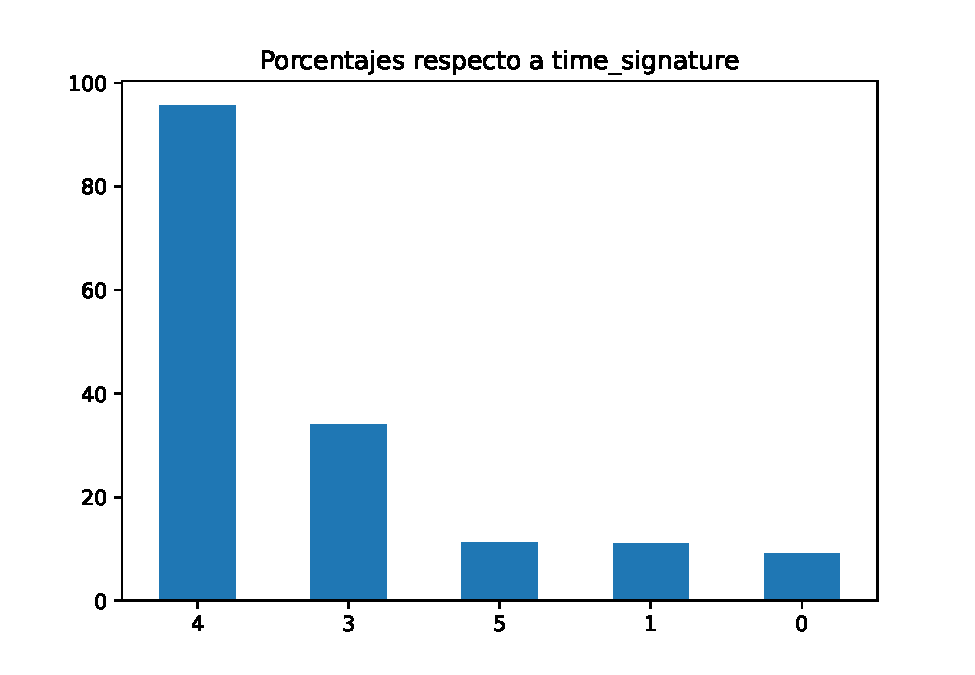
\includegraphics{informe_01_files/figure-pdf/unnamed-chunk-30-21.pdf}

\hypertarget{transformaciuxf3n-previa-a-la-imputaciuxf3n}{%
\subsubsection{Transformación previa a la
imputación}\label{transformaciuxf3n-previa-a-la-imputaciuxf3n}}

Las variables \textbf{duration\_ms}, \textbf{speechiness} e
\textbf{instrumentalness} requirieron ser transformadas vía la función
logaritmo, tras haber aumentado los valores en tales variables en 0.001,
para evitar valores 0, lo cual nos permite aplicar logaritmo. Ese
aumento de 0.001 se realizó porque aquellas tres variables poseen
valores entre 0 y 100.

\hypertarget{tratamiento-de-datos-atuxedpicos}{%
\subsubsection{Tratamiento de datos
atípicos}\label{tratamiento-de-datos-atuxedpicos}}

Se realizaron \textbf{Q-Q plots} para las variables numéricas, y se
observó que ninguna de aquellas variables seguía una distribución
gaussiana. Por ello, en vez considerar los whiskers superior e inferior
usuales, creamos una aplicación web con el fin de definir, de manera
interactiva, tales whiskers superior e inferior, bajo la condición que
los datos atípicos que producirían tales nuevos whiskers representen
menos del 10\% de la variable; así hicimos, variable por variable
(numérica).

Después de este paso, realizamos graficos de densidad para conocer las
distribuciones e identificar los valores ouliers. Los graficos nos
ayudaron a observar que, se hubiera perdido información importante en
caso se hubiera usado los whisker usuales ─que se generan asumiendo una
distribución normal─ debido a que estos cortaban en lugares que no
representaban valores atípicos reales para las distribuciones que tienen
las variables.

El siguiente paso es realizar la imputación de variables, para esto,
primero se intentó imputar la mediana a los valores atípicos, pero al
analizar las variables descubrimos que, las distribuciones de las
variables imputadas cambiaban notablemente; por lo tanto, este método
inicial quedó descartado. Luego, se eligió imputar mediante el algoritmo
de KNNimputer el cual se considera un método robusto para imputar
valores faltantes debido a que usa inforación de los k-vecinos más
cercanos para hallar el dato faltante.

Como primer paso para usar este método se tuvo que reemplazar todos los
valores atípicos con vacios, posteriormente se eligieron los parámetros
de la función KNNimputer, estos fueron: - n\_neighbors: 5, representa al
número de muestras vecinas a utilizar para la imputación - weights:
``uniform'', todos los pesos de cada vecino se ponderan por igual -
metric: nan\_euclidean, se utilizó la distancia euclidiana

Se intentó usar el algoritmo para todas las columnas numéricas a la vez,
pero este tomaba mucho tiempo en su ejecución debido a la cantidad de
datos, por eso, decidimos imputar las valores atípicos agregando solo
una columna con datos por imputar a la vez. Cuando finalizó todo este
proceso comprobamos que nuestra data no contenía vacios, indicador de
que funcionó correctamente el algoritmo.

Para considerar que esta imputación fue la adecuada usamos dos métodos.
Primero el test Kolmogorov-Smirnov que sirve para comparar la
distribución de dos conjuntos de datos, comparamos entonces el conjunto
de datos antes y después de imputar, pero el resultado no fue le
esperado porque obtuvimos que las distribuciones no eran iguales. En ese
momento nos planteamos cambiar nuevamente el método para imputar, pero,
antes de esto realizamos gráficos de densidad superpuestos para ambas
distribuciones y nos dimos cuenta que las distribuciones no tenían un
gran cambio; por lo tanto aceptamos este método como adecuado y
utilizamos la data imputada que obtuvimos en los siguientes pasos.

\hypertarget{tratamiento-de-datos-vacuxedos}{%
\subsubsection{Tratamiento de datos
vacíos}\label{tratamiento-de-datos-vacuxedos}}

Solamente en la variable \textbf{names} existen valores vacíos, 71, en
particular. Sin embargo, como se comentó previamente, tal columna se
descartará del dataset, pues existe otra columna que produce la misma
información que la columna \textbf{names} y que no presenta vacíos.

\hypertarget{creaciuxf3n-y-transformaciuxf3n-de-variables}{%
\subsubsection{Creación y transformación de
variables}\label{creaciuxf3n-y-transformaciuxf3n-de-variables}}

Debido a que inicialmente la base de datos con la que contábamos tenía
una reducida cantidad de columnas, de las cuales algunas no aportaban
con información relevante para el objetivo del negocio. En ese sentido,
transformamos las variables name, time\_signature y realice\_data. De
las cuales obtenemos información que podrán servir para la predicción.

\hypertarget{name}{%
\paragraph{Name}\label{name}}

Contiene el nombre de la canción, a partir de esta se generan dos
variables:

\begin{itemize}
\tightlist
\item
  Name\_lenght : contabiliza al cantidad de caracteres string del nombre
  de la canción omitiendo los espacios vacíos entre palabra y palabra.
\item
  Words\_name: contabiliza la cantidad de palabras que están presentes
  en el nombre de una canción.
\end{itemize}

Es importante recordar, que luego de generar ambas variables, se tiene
que eliminar la variable ``name'' para no caer en el problema de
multicolinealidad.

\hypertarget{release-date}{%
\paragraph{Release date}\label{release-date}}

Indica la fecha del lanzamiento de la canción incluyendo el año, mes y
día. Apartir de esat variable se crearon cuatro variables:

\begin{itemize}
\tightlist
\item
  Release\_year: año en el que se publicó la canción
\item
  Release\_month: mes en el que se publicó la canción
\item
  Release\_days: día en el que se publicó la canción
\item
  Release\_trim: trimestre en el que se publicó la canción
\end{itemize}

Posteriormente, eliminamos la variable realise date.

\hypertarget{time-signature}{%
\paragraph{Time signature}\label{time-signature}}

Esta variable \textbf{ordinal} contiene la cantidad de pulsos en un
compás, para cada canción. Esta variable toma valores de 3 a 7, así que
la discretizamos para que tome el valor de 0 si los valores son mayores
iguales a 0 y menores que 4; y tome el valor de 1 si los valores toman
valores mayores iguales a 4.

Esta recategorización se basa en el hecho que casi todas las canciones
que existen actualmente en el mundo poseen un valor de 4 en
\textbf{time\_signature}.

\hypertarget{popularity}{%
\paragraph{Popularity}\label{popularity}}

Para clasificar a las canciones en las categorías \textbf{popular} y
\textbf{no popular}, se escogió el valor 40 como punto de corte.

Es decir, canciones con un valor de popularidad menor a 40 se asignaron
a 0 (no populares); caso contrario, tales canciones se asignan a 1
(populares).

\hypertarget{key}{%
\paragraph{Key}\label{key}}

La variable key representa el centro tonal de la canción, habiéndose así
12 opciones para casi todas las canciones que existen actualmente: 0, 1,
\ldots, 10, 11 .

Como el \textbf{círculo de quintas} es un concepto musical empleado en
casi todas las canciones existentes, agruparemos en 4 categorías, a los
valores de key, agrupándolos de 7 en 7, ya que esto representa centros
tonales lo más cercanos posibles en el círculo de quintas.

Como el valor 0 de \textbf{key} representa al centro tonal C (Do), el
caso más popular entre todas las canciones del planeta, agruparemos a
los valores de \textbf{key} vía las siguientes categorías:

{[}5, 0, 7{]} =\textgreater{} 0

{[}8, 3, 10{]} =\textgreater{} 1

{[}11, 6, 1{]} =\textgreater{} 2

{[}2, 9, 4{]} =\textgreater{} 3

\hypertarget{descripciuxf3n-de-variables-listas-para-el-modelamiento}{%
\subsubsection{Descripción de variables listas para el
modelamiento}\label{descripciuxf3n-de-variables-listas-para-el-modelamiento}}

Variables utilizadas en el análisis estadístico:

\begin{longtable}[]{@{}
  >{\centering\arraybackslash}p{(\columnwidth - 4\tabcolsep) * \real{0.3333}}
  >{\centering\arraybackslash}p{(\columnwidth - 4\tabcolsep) * \real{0.3333}}
  >{\centering\arraybackslash}p{(\columnwidth - 4\tabcolsep) * \real{0.3333}}@{}}
\toprule
\begin{minipage}[b]{\linewidth}\centering
variable
\end{minipage} & \begin{minipage}[b]{\linewidth}\centering
clasificación
\end{minipage} & \begin{minipage}[b]{\linewidth}\centering
detalle
\end{minipage} \\
\midrule
\endhead
duration\_ms & numérica & - \\
explicit & numérica & - \\
release\_trim & categórica & Trimestre del año en que fue lanzada la
canción. \\
release\_day & categórica & Día del año en que fue lanzada la
canción. \\
release\_month & categórica & Mes del año en que fue lanzada la
canción. \\
words\_name & categórica & Número de palabras que tiene el nombre de la
canción. \\
Name\_Length & categórica & Cantidad de carácteres que tiene el nombre
de la canción. \\
time\_signature & categórica & 0 si hay de 0 a 3 pulsos en cada compás y
1 cuando existe más de 3 pulsos. \\
mode & categórica & Indica la modalidad (1) o menor (0) de una pista. \\
tempo & numérica & - \\
danceability & numérica & - \\
valence & numérica & - \\
liveness & numérica & - \\
instrumentalness & numérica & - \\
acousticness & numérica & - \\
speechiness & numérica & - \\
loudness & numérica & - \\
energy & numérica & - \\
list\_key & categórica & List key agrupa los centros tonales de las
canciones, donde 0 representa el centro tonal C(Do), 1 representa Re, 2
representa Mi y finalmente 3 representa Fa. \\
\bottomrule
\end{longtable}

Con las variables listas para modelar hacemos un análisis descriptivo de
las variables numéricas.

\begin{longtable}[]{@{}
  >{\centering\arraybackslash}p{(\columnwidth - 16\tabcolsep) * \real{0.1111}}
  >{\centering\arraybackslash}p{(\columnwidth - 16\tabcolsep) * \real{0.1111}}
  >{\centering\arraybackslash}p{(\columnwidth - 16\tabcolsep) * \real{0.1111}}
  >{\centering\arraybackslash}p{(\columnwidth - 16\tabcolsep) * \real{0.1111}}
  >{\centering\arraybackslash}p{(\columnwidth - 16\tabcolsep) * \real{0.1111}}
  >{\centering\arraybackslash}p{(\columnwidth - 16\tabcolsep) * \real{0.1111}}
  >{\centering\arraybackslash}p{(\columnwidth - 16\tabcolsep) * \real{0.1111}}
  >{\centering\arraybackslash}p{(\columnwidth - 16\tabcolsep) * \real{0.1111}}
  >{\centering\arraybackslash}p{(\columnwidth - 16\tabcolsep) * \real{0.1111}}@{}}
\toprule
\begin{minipage}[b]{\linewidth}\centering
variable
\end{minipage} & \begin{minipage}[b]{\linewidth}\centering
count
\end{minipage} & \begin{minipage}[b]{\linewidth}\centering
mean
\end{minipage} & \begin{minipage}[b]{\linewidth}\centering
std
\end{minipage} & \begin{minipage}[b]{\linewidth}\centering
min
\end{minipage} & \begin{minipage}[b]{\linewidth}\centering
0.25
\end{minipage} & \begin{minipage}[b]{\linewidth}\centering
0.5
\end{minipage} & \begin{minipage}[b]{\linewidth}\centering
0.75
\end{minipage} & \begin{minipage}[b]{\linewidth}\centering
max
\end{minipage} \\
\midrule
\endhead
popularity & 586672 & 27.570053 & 18.370642 & 0 & 13 & 27 & 41 & 100 \\
duration\_ms & 580069 & 5.323873 & 0.165679 & 4.700011 & 5.245019 &
5.332467 & 5.420505 & 5.899967 \\
danceability & 586343 & 0.563908 & 0.165612 & 0.0532 & 0.453 & 0.577 &
0.686 & 0.988 \\
energy & 586672 & 0.542036 & 0.251923 & 0 & 0.343 & 0.549 & 0.748 & 1 \\
loudness & 584103 & -10.114038 & 4.855248 & -29.999 & -12.838 & -9.22 &
-6.474 & -0.004 \\
speechiness & 563644 & -1.259542 & 0.284709 & -1.645892 & -1.459671 &
-1.354578 & -1.154282 & -0.185087 \\
acousticness & 586672 & 0.449863 & 0.348837 & 0 & 0.0969 & 0.422 & 0.785
& 0.996 \\
instrumentalness & 562639 & -2.441072 & 0.951667 & -3 & -3 & -2.993235 &
-2.295849 & -0.050122 \\
liveness & 563897 & 0.188345 & 0.134634 & 0 & 0.0969 & 0.134 & 0.253 &
0.7 \\
valence & 586672 & 0.552292 & 0.257671 & 0 & 0.346 & 0.564 & 0.769 &
1 \\
tempo & 585134 & 118.585417 & 29.438423 & 50.002 & 95.757 & 117.4715 &
136.33 & 210 \\
\bottomrule
\end{longtable}

\hypertarget{capuxedtulo-iv-desarrollo-del-modelo}{%
\subsection{CAPÍTULO IV: DESARROLLO DEL
MODELO}\label{capuxedtulo-iv-desarrollo-del-modelo}}

Escogemos la gama de modelos de clasificación para cumplir con el
objetivo del proyecto. En el presente trabajo trabajamos con tres
modelos teóricos:

\begin{itemize}
\tightlist
\item
  Árbol de clasificación CART
\item
  Regresión logística
\item
  Random Forest Classifier
\end{itemize}

Sin emabargo, hacemos combinaciones de estos tres modelos con los tipos
de balanceo (undersample y oversample)y grid search, de forma que
finalmente evaluamos 10 modelos de clasificación.

Por otro lado, luego de pre procesar los datos decidimos eliminar la
variable ``year\_release, pues no es de utilidad como variable
predictora porque el modelo se usará en el futuro para classificar
canciones del 2022, en adelante. De esa forma, los nuevos años que se
integren a la data podrían ser considerados como valores atípicos.

\hypertarget{anuxe1lisis-de-correlaciuxf3n-entre-variables}{%
\subsubsection{Análisis de correlación entre
variables}\label{anuxe1lisis-de-correlaciuxf3n-entre-variables}}

Se observa que los colores que adoptan las casillas de la matriz de
correlación son rosados, lo cual indica que las variables tienen un
coeficiente de correlación que se encuentra entre 0.2 y 0.4, es decir el
nivel de correlación entre variables numéricas predictoras no es muy
alta.

\hypertarget{particiuxf3n-en-datos-de-train-test-o-train-test-val}{%
\subsubsection{Partición en datos de train-test (o
train-test-val)}\label{particiuxf3n-en-datos-de-train-test-o-train-test-val}}

Nuestro dataset, fue dividido en grupos aleatorios más pequeños para que
estos puedan ser utilizados posteriormente por los conjuntos de
entrenamiento(train), testeo(test) y validación(val).Para esta partición
de datos utilizamos el algoritmo de train\_test\_split e indicamos que
la partición se haga por la cuarta parte de la cantidad de registros
original. De esta forma, el grupo de entrenamiento representó el 75\% de
la data y el conjunto de testeo representó el 25\% de la data.

\hypertarget{balanceo-de-datos-en-caso-aplique}{%
\subsubsection{Balanceo de datos (en caso
aplique)}\label{balanceo-de-datos-en-caso-aplique}}

Popularidad es la variable dependiente de nuestro interes, la cual,
luego de una transformación de variable, adquirió solo dos valores: 0 y
1. 0 en caso la canción no sea popular, y 1 en caso contrario.
Observamos que el 73\% de los valores son 0 ─no populares─ y el 27\% de
los valores son 1 ─populares─, lo cual podría influenciar en los
resultados que muestren nuestros modelos analíticos. En este escenario,
concluimos que era necesario realizar balanceo de datos.

Para el balanceo de datos, decidimos usar dos tipos de balanceo:
undersampling y oversampling. Por un lado en la estrategia
undersampling, usamos el algoritmo \textbf{RandomUnderSampler} para
eliminar los registros de canciones que no son populares, quedandonos
con una cantidad de registros igual a la cantidad de registros que son
populares. Por otro lado, en la estrategia oversampling, usamos el
algoritmo \textbf{Smote} para agregar registros de canciones que son
populares, quedandonos con una cantidad de registros igual a la cantidad
de registros que no son populares. Antes de realizar el balanceo
verificamos también si los registros contaban con vacíos, al no ser el
caso se procedió a crear dos nuevos conjuntos de datos
``x\_train\_smote'' y ``y\_train\_smote'' para el caso del balanceo de
datos usando el algoritmo \textbf{Smote}, y se creó los conjuntos de
datos ``x\_resampled'' y ``y\_resampled'' para el caso del balanceo de
datos usando el algoritmo \textbf{RandomUnderSampler}, estos nuevos
conjuntos balanceados fueron utilizados posteriormente para probar
modelos.

\hypertarget{selecciuxf3n-de-paruxe1metros-en-caso-aplique}{%
\subsubsection{Selección de parámetros (en caso
aplique)}\label{selecciuxf3n-de-paruxe1metros-en-caso-aplique}}

La elección de los parametros fue de dos formas, en primer lugar, en el
primer y cuarto modelo de estableció lo parametros, pero en el caso de
los demás modelos se utilizó \textbf{GridSearchCV}, el cual es un
algortimo que ayuda a elegir los hiperparámetro óptimos para un modelo,
en el caso de los árboles de clasificación y bosque aleatorio, este nos
ayuda a poder las ramas de los árboles para que estos no sean tan
profundos. A continuación, se incluye una tabla resumen de los
parametros que finalmente se usaron en los modelos. Es importante notar,
que el algoritmo de optimización de parametros recomienda usar el
indicador de entropia para la partición de los nodos, en caso de que el
modelo sea un árbol de clasificación.

\begin{longtable}[]{@{}
  >{\centering\arraybackslash}p{(\columnwidth - 4\tabcolsep) * \real{0.3333}}
  >{\centering\arraybackslash}p{(\columnwidth - 4\tabcolsep) * \real{0.3333}}
  >{\centering\arraybackslash}p{(\columnwidth - 4\tabcolsep) * \real{0.3333}}@{}}
\toprule
\begin{minipage}[b]{\linewidth}\centering
Modelos
\end{minipage} & \begin{minipage}[b]{\linewidth}\centering
Grid Search
\end{minipage} & \begin{minipage}[b]{\linewidth}\centering
Hiperparámetros
\end{minipage} \\
\midrule
\endhead
Árbol de clasificación CART & No & semilla aleatoria, índice de Gini \\
Árbol de clasificación CART & Si & semilla aleatoria, índice de Gini \\
Árbol de clasificación CART & Si & semilla aleatoria, índice de
entropia, splitter: best \\
Regresión Logística & No & max\_inter:200, semilla aleatoria \\
Regresión Logística & Si & max\_inter:200, semilla aleatoria \\
Árbol de clasificación CART & Si & semilla aleatoria, índice de Gini \\
Árbol de clasificación CART & Si & `criterion': `entropy',
`random\_state': 0, `splitter': `best' \\
Regresión Logística & Si & `max\_iter': 200, `random\_state': 0 \\
Random Forest Classifier & Si & `criterion': `entropy', `random\_state':
0 \\
Random Forest Classifier & Si & `criterion': `entropy', `random\_state':
0 \\
\bottomrule
\end{longtable}

\hypertarget{selecciuxf3n-del-mejor-modelo}{%
\subsubsection{Selección del mejor
modelo}\label{selecciuxf3n-del-mejor-modelo}}

En indicador \textbf{accuracy} indica qué tan bien predice el modelo, el
indicador de \textbf{sensibilidad} evalúa que tan bien se clasifica a
las canciones populares y el indicador de \textbf{especificidad} evalúa
que tan bien se clasifica a las canciones no populares.

En la siguiente tabla, se observa el resultado de los modelos evaluados
en el conjunto de testeo. Se observa que los modelos 4, 8 y 9 registran
valores altos en el indicador especificicidad, esto indica que estos
modelos clasifican bien en las canciones no pupulares en mas del 90\% de
casos. Po rlo cual descartamos estos modelos, ya que nuestro objetivo es
clasificar canciones populares. De esta forma, consideramos que el
modelo que presente un porcentaje más alto en el indicador de
\textbf{sensibilidad} es el modelo que clasifica mejor las canciones
populares. Como se observa, el modelo 5: modelo de regresión logística
con balanceo de datos \textbf{SMOTE} y \textbf{GridSearchCV} es el
modelo que presenta un mejor resultado en el indicador de
\textbf{sensibilidad}, pues clasifica bien a las canciones populares en
el 75\% de casos.

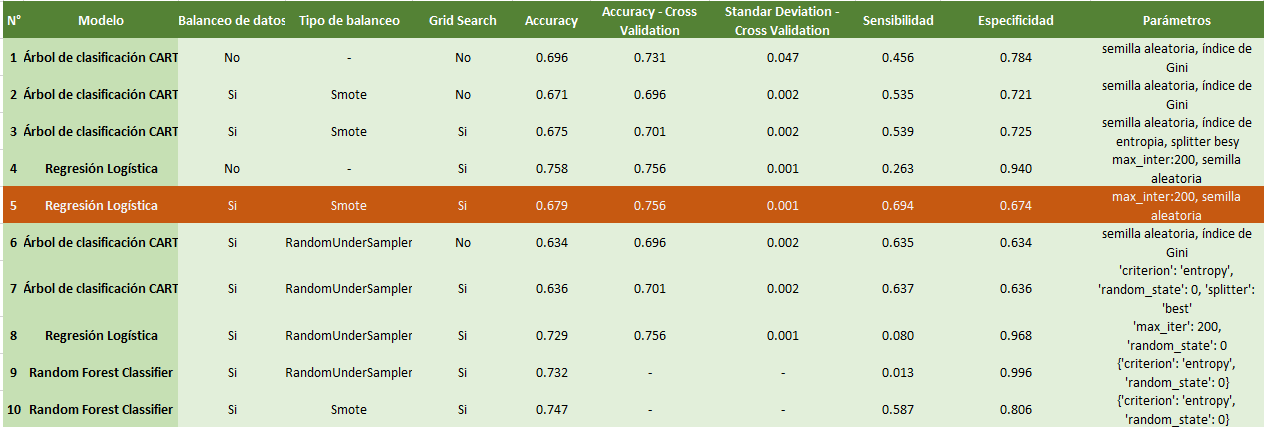
\includegraphics[width=4.21in,height=\textheight]{comparacion-modelos.png}

Por otro lado, a continuacion se observa una tabla de resumen de la
regresión logistica evaluada sobre el conjunto de testeo. Se observa que
existe significancia conjunta y significancia individual en todas las
variables individuales. Asimismo, observamos que la variable
\textbf{danceability} y \textbf{loudness} es la variable que impacta de
forma altamente positiva sobre la variable dependiente, esto quiere
decir que cuanto mas bailable sea la canción, mas popular será. Sin
emabrgo, nos parece sospechoso que al variable cantidad de palabras
tenga un coefiente muy alto y positivo, pues se esperaría que el cuanto
menos palabras tenga la cancion sea mas popular.

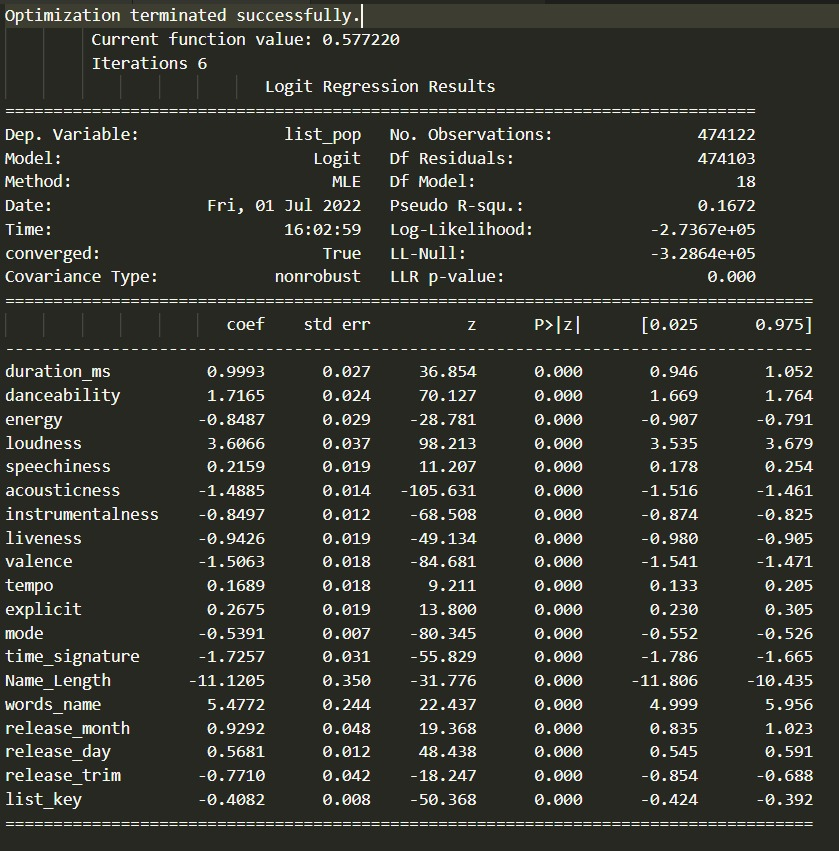
\includegraphics{mejor-modelo.jpg}

\hypertarget{descripciuxf3n-de-la-estructura-del-modelo-seleccionado}{%
\subsubsection{Descripción de la estructura del modelo
seleccionado}\label{descripciuxf3n-de-la-estructura-del-modelo-seleccionado}}

El modelo escogido es entrenado con el algoritmo de regresión logística
con el balanceo de datos \textbf{SMOTE}, con los siguientes parámetros:
max\_inter:200, semilla aleatoria, lo cuales fueron elegidos por
\textbf{GridSearchCV}. Los modelos de regresión logistica tratan de
predecir la clasificacion de las categorias de la variable dependiente,
en este caso, la variable \textbf{popularity}. El cual esa el metodo de
estimación de maxima verosimilitud para cacular sus resultados, asi
mismo, al ser unre gresion lineal las variables independientes pueden
ser intepretads en signos y probabildad.

\hypertarget{capuxedtulo-v-conclusiones}{%
\subsection{CAPÍTULO V: CONCLUSIONES}\label{capuxedtulo-v-conclusiones}}

En conclusión, el modelo de regresión logítica es el modelo que presenta
un mejor resultado en el indicador de \textbf{sensibilidad}, pues
clasifica bien a las canciones populares en el 75\% de casos, donde se
observa que la bailabilidad y \textbf{loudness} es la variable que
impacta positivamente sobre la popularidad de una canción. No obstante,
hay algunas variables que no tienen el signo esperado, como la variable
cantidad de palabras, pues se esperaría que el cuanto menos palabras
tenga, la canción sea más popular. Definitivamente, el análisis
individial de las variables en el modelo de regresión debe ser
supervisado por un experto del negocio.

\hypertarget{capuxedtulo-vi-recomendaciones}{%
\subsection{CAPÍTULO VI:
RECOMENDACIONES}\label{capuxedtulo-vi-recomendaciones}}

\begin{itemize}
\tightlist
\item
  El dataset con el que trabajamos, que fue descargado de Kaggle,
  presentaba diversos problemas:

  \begin{itemize}
  \tightlist
  \item
    Esta consistía principalmente de canciones no populares, así que los
    modelos trabajados predecían \textbf{no popularidad}, en vez de
    popularidad.
  \item
    Esta contiene una fila con data errónea, pues a una banda chilena se
    le asignan valores incorrectos respecto a la fecha de publicación de
    las canciones. Por ello, recomendamos que se utilice el
    identificador Spotify de las canciones del dataset, para scrapear la
    información actualizada de tales canciones. Además, añadir canciones
    populares al dataset, para que los modelos a emplearse puedan
    predecir \textbf{popularidad}, a partir de una data mejor balanceada
    respecto a canciones populares y no populares.
  \end{itemize}
\end{itemize}

\end{document}
